
\documentclass{sig-alternate}

\begin{document}
%
% --- Author Metadata here ---
\conferenceinfo{18-697}{Fall '14 Pittsburgh, PA USA}
\CopyrightYear{2014}
% --- End of Author Metadata ---

\title{Clustering for Controlling Stochastic Optimization using Feedback}
\subtitle{Applied to Newspaper Article Title Category Prediction}

\numberofauthors{2} 
\author{
\alignauthor
Kevin Brennan\\
       \affaddr{Carnegie Mellon University}\\
       \affaddr{5000 Forbes Avenue}\\
       \affaddr{Pittsburgh, PA}\\
       \email{kbrennan@andrew.cmu.edu}
% 2nd. author
\alignauthor
Gavriel Adler\\
       \affaddr{Carnegie Mellon University}\\
       \affaddr{5000 Forbes Avenue}\\
       \affaddr{Pittsburgh, PA}\\
       \email{gya@andrew.cmu.edu}\\
}


\maketitle
\begin{abstract}
In optimizing feature sets for classification, there are often multiple local optima. In order to reduce complexity and computational cost, it is often desirable to deal with only a fixed number of solutions. One method for controlling the size of the solution set is with generalized crowding.\\
\indent In this paper, we explore using a genetic algorithm for creating optimized feature sets for classification problems. Through several trials of a genetic algorithm, we create a solution space of locally optimal feature sets. Using generalized crowding and K-Means clustering, we refine the solution space into a set of niches. Based on the difference between a desired number of niches and the number returned by the clustering algorithm, we implement a feedback controller for the exploration/exploitation of the genetic algorithm. By tuning this parameter, we adjust the range of the solution space through several iterations till it converges to the set point. After testing on classifying newspaper titles, the algorithm showed the controller to be ineffective in converging the solution space to a desired number of clusters. Control over the exploration/exploitation parameter did not have sufficient power to augment the number of niches for the given implementation.
\end{abstract}

\terms{Classification, Feedback, Stochastic Optimization}

\keywords{Controlled Clustering, Naive Bayes, K-Means, Title Category Classification}

\section{Introduction}
The problem of optimizing feature sets for use in classification is often multi-modal, with each local optima having its unique characteristics. Although multiple solutions often give a better representation of the solution space for a given optimization, having a variable number of solutions increases the complexity and cost of a given algorithm.\\
\indent One method for creating a fixed-size solution set is through crowding. Crowding groups elements of the current generation of the genetic algorithm based on a given fitness functions\cite{ole:feedback}. Using a scaling factor, generalized crowding controls the range of solutions  with respect to the given fitness function. In the case of evolutionary algorithms such as genetic algorithms, the scaling factor controls the exploration/exploitation parameter used in determining survival between generations. Control of the scaling factor therefore also controls the number of niches within a given solution space\cite{ole:feedback}.\\
\indent In this paper, we detail using genetic algorithm to optimize feature sets for classifying newspaper titles into topics. For classification, each feature set is a set of words. Through several trials of a genetic algorithm, we create a set of locally optimized feature sets. With each generation of the genetic algorithm, we use generalized crowding in order to control the solution set. The solution set is then clustered with K-Means. We apply a feedback controller on the error between the desired number of clusters and this returned number. In this paper, we consider the use a full PID controller in order to expand upon past research in this area. Using derivative and integral gains allows for greater control of the rate of convergence, overshoot, and steady state error when refining the number of  niches. Further information on the implementation of our algorithm is provided in the Algorithm section of our paper.  

\section{Background}
\subsection{Feature Selection}
In classification by feature set, the computation time and cost are directly linked to the number of features used. Each additional features increases the number of comparisons and therefore time to classification\cite{features}. The goal of feature selection is to minimize the number of features used while maintaining a certain degree of classification accuracy. In optimizing feature sets, it is possible to both change the size of the set and the combinations of features used. Since the problem is parameterized by multiple elements, the solution is often multi-modal. In addition, each parameter can be optimized with respect to the change in classification accuracy or the change in computation time.\\
\indent One method for handling this multi-modal problem is to use genetic algorithms\cite{features}. Genetic algorithms have the ability to explore multiple local optima, while also requiring minimal a priori knowledge. Genetic algorithms work by having several nodes, feature sets, compete for survival between generations of the algorithm. The survival of a given node is based on a fitness function. In addition to the fitness function, there are random mutations and cross-over in the nodes. The rate at which these events occur are based on parameterized probabilities. These event prevent premature convergence in the search for local optima and extend the range of the solution space\cite{galan:feedback}. One implementation for feature selection first converts each feature set to a bit-string\cite{features}. Each one in the bit-string indicates that a given feature from the overall feature is used by the current feature set. Based on this relationship, one can then calculate a similarity index between two feature sets based the features used in both. The fitness function for this given implementation is based on the classification scores for each feature set. The nodes which survive between generations are then generally the ones with the higher classification scores.

\subsection{Generalized Crowding for Genetic Algorithms}
Crowding is a method of determining survival in a genetic algorithm based on a selective pressure. The selective pressure determines the survivor for each competition between child and parent\cite{galan:feedback}. Generalized Crowding expands upon Crowding by parameterizing the selective pressure\cite{galan:feedback}. This parameterization is known as the scaling factor or $\phi$ term. It controls the degree to which the algorithm values exploration over exploitation in the survival stages between generations\cite{galan:feedback}. Controlling this factor extends the range of the solution space because it allows for non-optimal survivors between generations. This method decreases the likelihood of the nodes converging to a single local optima, and thereby explores more of the possible solutions.

\section{Algorithm}
\begin{figure*}[t]
\centering
\fbox{
  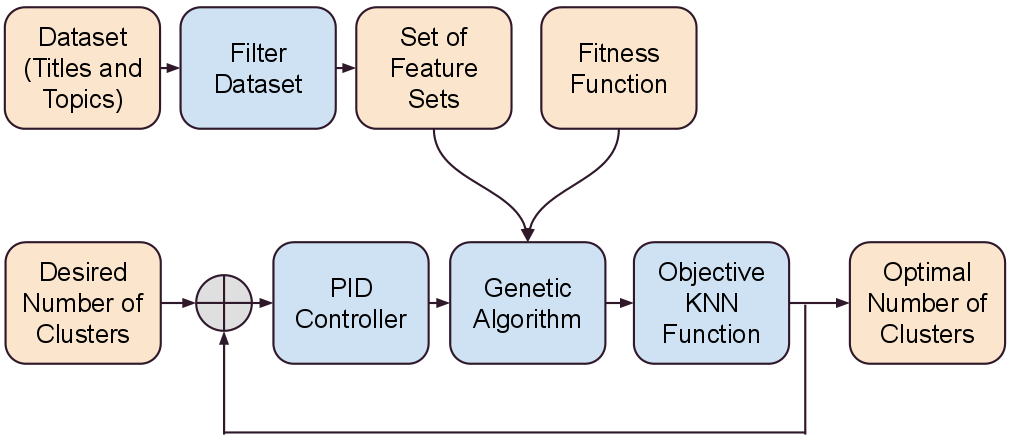
\includegraphics[width=0.8\textwidth]{pipeline.png}}
\caption{The Algorithm Pipeline}
\label{fig:pipeline}
\end{figure*}
\subsection{Pipeline Overview}
Our pipeline, as seen in Figure~\ref{fig:pipeline}, consists of a few independent pieces put together in a control loop. To initialize the pipeline, we first separated the titles into a training and a testing set. We then made a list of words that appear in the titles of the training set and filtered the data set into our feature sets, or sets of bags of words from that list. In the control loop, we get our error value from the difference between the optimal number of clusters returned by the objective K-Means function and the desired number of clusters. The error and the PID controller created a $\phi$ term representing exploration vs. exploitation. We generated sets of bags of words from the training set list and passed each into the genetic algorithm along with the $\phi$ term, and each returned a locally optimal bag of words. These optimal bags were clustered to find the optimal number of clusters, and the loop restarts. Each section of the algorithm is discussed in detail below.

\subsection{Genetic Algorithm}
\begin{figure}[t]
\centering
\fbox{\rule{0pt}{2in}
  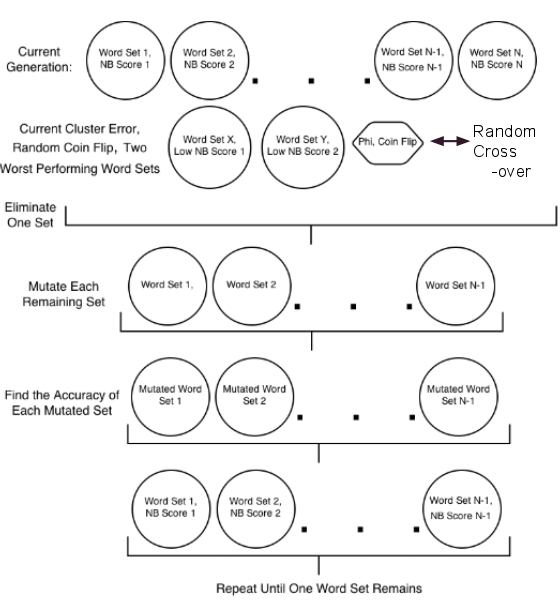
\includegraphics[width=0.45\textwidth]{genetic_algo.png}}
\caption{The flow of one iteration of the genetic algorithm}
\label{fig:genetic_algo}
\end{figure}
Our genetic algorithm operated on a set of bags of words, and converges to a single locally optimal bag of words. At each round of the genetic algorithm, the Naive Bayes score on the testing set was calculated for each bag of words. The lowest two scores competed for survival, and the victor was based on both the $\phi$ exploration/exploitation term and a random coin flip. After one bag was killed, each remaining bag was mutated and additional randomized cross-over between trials was added in to further diversity. Our solution set was created by running several trials of the genetic algorithm on many randomly generated sets of bags of words.\\
\indent In the mutation step, the algorithm attempted to replace each word in the bag of words with a new word taken from the titles in the training set. If the Naive Bayes score of the bag of words with the new word was higher than it was with the old word, the new word replaced the old word, otherwise the new word was discarded.\\
\indent This process of testing with Naive Bayes continues till only a single bag of words is left. We add this bag of words to our solution set, and after all the trials of the genetic algorithm are finished we have a set locally optimal solutions. This solution set is then passed onto the clustering algorithm.

\subsection{Clustering Algorithm}
Our clustering algorithm is based on the Objective K-Means function. The objective function works by running K-Means with a variable number of nodes used for clustering. For each element of the solution set created by the genetic algorithm trials, we calculate the number of true positives, false positives, true negatives, and false negative. A true positive or true negative represents the correct classification of a title, and conversely a false positive or false negative represents a failure to do so. This representation is possible because we are separating the titles into only two classes. We used these statistics, instead of other distance metrics such as the Hamming distance as used in previous research\cite{ole:feedback}, in order to cluster the solutions by characteristics. For instance, to have a group of solutions with minimal false positives or another with minimal false negatives.\\
\indent Based on these statistics, we calculate a distance to each node based on the Euclidean distance metric. For K-Means, we group each element to the closest node, and re-calculate a mean node for each grouping. K-Means continues to iterate until the mean nodes remain constant between iterations. Once K-Means finishes iterating, we calculate the distance of each element to its group's mean node. The sum of these distances is our error for that given number of nodes.\\
\indent Based on the error for each number of nodes, we find the change in the error with respect to the change in the number of nodes. This change is the first derivative of the error. Next, we find the change in the first derivative with respect to the change in the number of nodes. This change is the second derivative of the error. The elbow point for the errors is then calculated by the maximum second derivative. For our feedback loop, the elbow point returned by our clustering algorithm represents the optimal number of nodes, or local optima, to use.

\subsection{Feedback Controller}
For controlling $\phi$ for the genetic algorithm, we use a PID controller. The set point for the controller is the desired number of clusters. The error is the difference between the set point and the returned number of clusters from the clustering algorithm. Based on this error, we calculate the change in the exploration/exploitation term for the next iteration of the feedback loop. The change is determined by calculating the change in error between iterations of the feedback loop, which is our derivative term, and the sum of all past errors, which is our integral term. By multiplying these terms and the error by set gains, we calculate the new exploration/exploitation term. The goal of implementing a full PID controller is to improve upon the efficiency of the entire pipeline by reducing the number of iterations till convergence to the desired number of clusters. The derivative term should improve the responsiveness of the controller while the integral term should ensure that the limit of the error goes to zero in time.

\subsection{Implementation}
We implemented our pipeline using Python's PANDAS module. Python, a scripting language, is easy to work with and develop quickly which was important given the project had to be finished within a semester. PANDAS is built on top of Python's NumPy library, which is strictly typed and invokes C calls, significantly speeding up the slow execution of Python. Lastly, we implemented clustering using Python's scikit-learn library, a machine learning library. Scikit-learn is also built in NumPy, making passing data between the two libraries very simple. In the end we were able to run our pipeline very efficiently, with each iteration of the feedback loop taking on the order of seconds instead of minutes. This speed allowed us to try many different runs of various combinations of parameters and analyze the results.

\section{Experiments}
\subsection{Data}
For our experiments, we used the Boydstun New York Times Front Page Data Set\cite{boydstun}. The data set contains every NYT front page article title from 1/1/1996 through 12/31/2006. The data set used ten different categories for classification. Each title can be marked as one or none of the given categories. In order to limit our algorithm to two topics, we chose "War on Terror" and "Presidential Elections". These two topics were chosen because they are similar enough that classifying titles a either one becomes a significant challenge and different enough that it is possible to differentiate between the two. Based on these two topics, we filtered the data set by removing any titles that did not fit into either of these two topics. Based on the remaining titles, we created a bag of words or bit-strings. With this bag of words, we create randomized sets of words with each set being a fixed size. These sets are the feature sets used in the later classification stages of the algorithm.
 
\subsection{Results}
In testing, we experimented with different controller gains, number of features per feature set, and number of trials of the genetic algorithm. For data, we recorded the clustering error per each number of niches used, the number of niches returned by the objective clustering algorithm, and the $\phi$ term, for each iteration of the control loop.
\begin{figure}[t]
\centering
\fbox{\rule{0pt}{2in}
  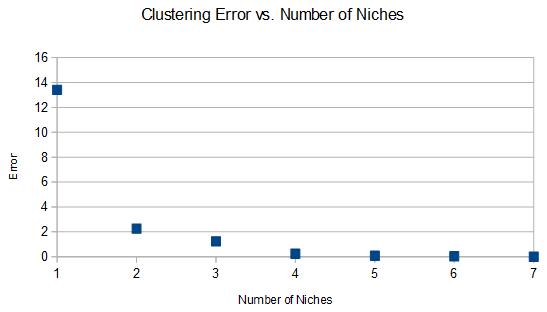
\includegraphics[width=0.45\textwidth]{graph2.png}}
\caption{A sample of the clustering error versus number of niches created by the clustering algorithm.}
\label{fig:graph1}
\end{figure}
A sample representation of the objective clustering algorithm is shown in Figure 3. The graph shows how well the solution set clustered given a certain number of nodes for clustering. Based on this error, we calculate the first and second derivatives of the error with respect to number of niches used for clustering. Our algorithm determines the optimal number of niches to be the point with the maximum second derivative. The result of the iteration displayed in this graph is two niches for clustering. This graph is representative of the majority of the trials of our entire algorithm. Even through varying the $\phi$ term and the number of words per set, overall the number of niches remains at 2. This result is shown in Figure 4.
\begin{figure}[t]
\centering
\fbox{\rule{0pt}{2in}
  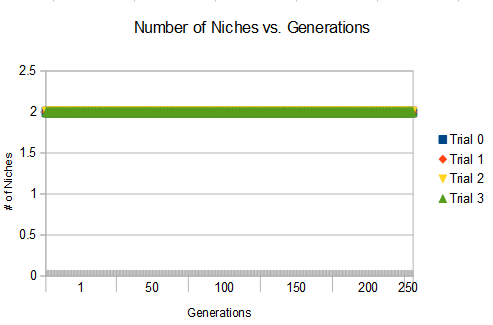
\includegraphics[width=0.45\textwidth]{graph1.png}}
\caption{The number of niches chosen by the clustering algorithm across the iterations of the feedback loop.}
\label{fig:graph2}
\end{figure}
Figure 4 shows the output of the control loop after each generation for several different trials. Trial 0 is the baseline with a proportional controller with a gain of 0.01 and five bit-strings per feature set. Trial 1 is with a proportional and derivative controller with gains of 1 and 0.1 and five bit-strings per feature set. Trial 2 is with the same controller as Trial 0, but with 10 bit-strings per feature set. Trial 3 is with the same controller as Trial 0, but with 15 bit-strings per feature set. The graph shows that the returned number of niches is invariant to these parameters. In addition, we noted that the classification accuracy remained constant at approximately seventy percent with a margin of 0.02. This accuracy is approximately equal to the score obtained when using our entire bag of words as a classifier. These results shows that not only does the number of niches not converge given changes to the $\phi$ term, but also that accuracy remains relatively consistent even with the reduction to only five bit-strings per feature set.\\
\begin{figure}[t]
\centering
\fbox{\rule{0pt}{2in}
  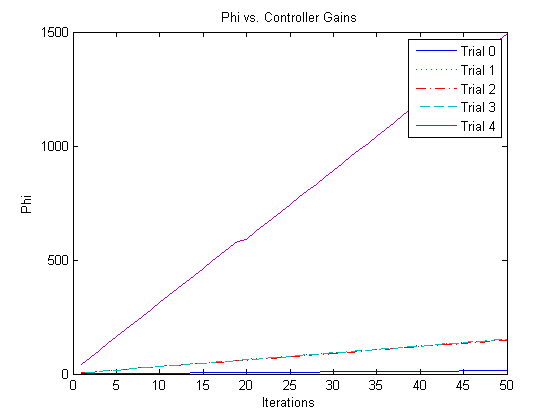
\includegraphics[width=0.45\textwidth]{graph3.png}}
\caption{The exploration/exploitation term over several iterations of the control loop.}
\label{fig:graph3}
\end{figure}
\begin{figure}[t]
\centering
\fbox{\rule{0pt}{2in}
  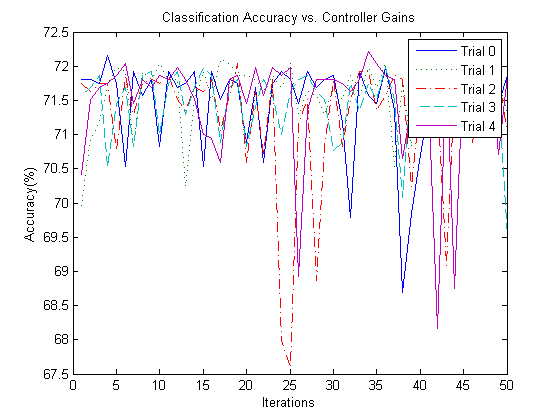
\includegraphics[width=0.45\textwidth]{graph4.png}}
\caption{The accuracy over several iterations of the control loop.}
\label{fig:graph3}
\end{figure}
\indent Figure 5 and Figure 6 show the results of our experiments with the controller gains. The experiments were run with the set point, desired number of clusters, as 4. Figure 5 shows the classification accuracy for each iteration of the control loop. Figure 6 shows the corresponding $\phi$ term used for the genetic algorithm based on the number of niches returned in the previous iteration. The parameters for each trial were:

\begin{center}
\begin{tabular}{ l | l | l | l }
  Trial & P & I & D \\ \hline
  $0$ & $0.1$ & $0$ & $0$  \\
  $1$ &   $1$ & $0$ & $0$ \\
  $2$ &   $1$ & $0$ & $0.1$ \\
  $3$ &   $1$ & $0.001$ & $0.1$  \\
  $4$ &  $10$ & $0$ & $0.5$ 
\end{tabular} \\
\end{center}


The results shows that the classification accuracy is invariant of the controller. Coupled with the results in Figure 4, this graph also shows that the $\phi$ term does not have a significant impact on the convergence in the number of niches. Figure 6 show $\phi$ term has a constant increase. This consistency is due to the fact that the error from each iteration controls the change in $\phi$ for the next iteration. Since the error is consistent, the change in $\phi$ is consistent.\\
\indent Based on all the results shown above, we conclude that the controller had minimal impact on the genetic algorithm. Although the number of clusters did not converge, we cannot conclude that the controller does not have an impact on the efficiency of the algorithm. Instead, the results suggest that further experimentation with additional optimization algorithms is needed to fully test the possibilities of a feedback controller. In addition, the results show that with a given fitness function, we may not be guaranteed to converge to desired number of clusters or optimal solutions. 

\section{Conclusion and Future Work}
This paper details the use of genetic algorithm, clustering, and feedback control in order to fixed-size optimized feature sets for classification. A PID controller adjusts the parameters of the genetic algorithm in order to control the range of the solution space. Clustering groups the solution space into a set of niches. This set of niches determines the error for the control loop in the next iteration of the feedback loop. This paper explores the use of derivative and integral terms in order to increase the responsiveness of the controller. In addition, it explore the use of different distance metrics used for clustering in order to investigate the characteristics of each of the solution space's niches. Although the results did not yield great success in controlling the solution space, the work detailed leaves several areas for further investigation and experimentation.\\
\indent For future work, we would experiment with other distance metrics for clustering. As mentioned in the results section, the classification results proved to be similar to create substantial differences in clustering. This similarity caused the solution set to sometimes converge to a single cluster, which impede the feedback controller. One potential alternative would be to represent the feature set as a bit-string and use the Hamming distance as a similarity index\cite{features}\\
\indent Another area for future work would be the creation of classification rules in the genetic algorithm. In our current algorithm, we rely solely on Naive Bayes as the classifier for a given feature. We could expand upon our implementation by using decision trees based on the Naive Bayes results for each element of a given feature set. This expansion could improve the classification scores of the feature set as it considers combinations of words in a title rather just each word by itself.

\begin{thebibliography}{100}
	
	\bibitem{ole:feedback} Shi, J., Mengshoel, O.J., and Pal,D.K., "Feedback Control for Multi-modal Optimization using Genetic Algorithms," \emph{Carnegie Mellon University}.
	\bibitem{features} Vafaie, H. and Jong, K.D., "Genetic Algorithms as a Tool for Feature Selection in Machine Learning," \emph{Center for Artificial Intelligence, George Mason University}.
	\bibitem{galan:feedback} Galan, S.F., and Mengshoel, O.J, "Generalized Crowding for Genetic Algorithms," \emph{Carnegie Mellon University}.
	\bibitem{boydstun}The University of Texas at Austin. (2006). "Boydstun NYT Front Page Dataset". <http://www.policyagendas.org/document/boydstun-nyt-front-page-dataset>
	
\end{thebibliography}

\end{document}
